\documentclass{article}
\usepackage{amsmath}
\usepackage{tikz}

\begin{document}

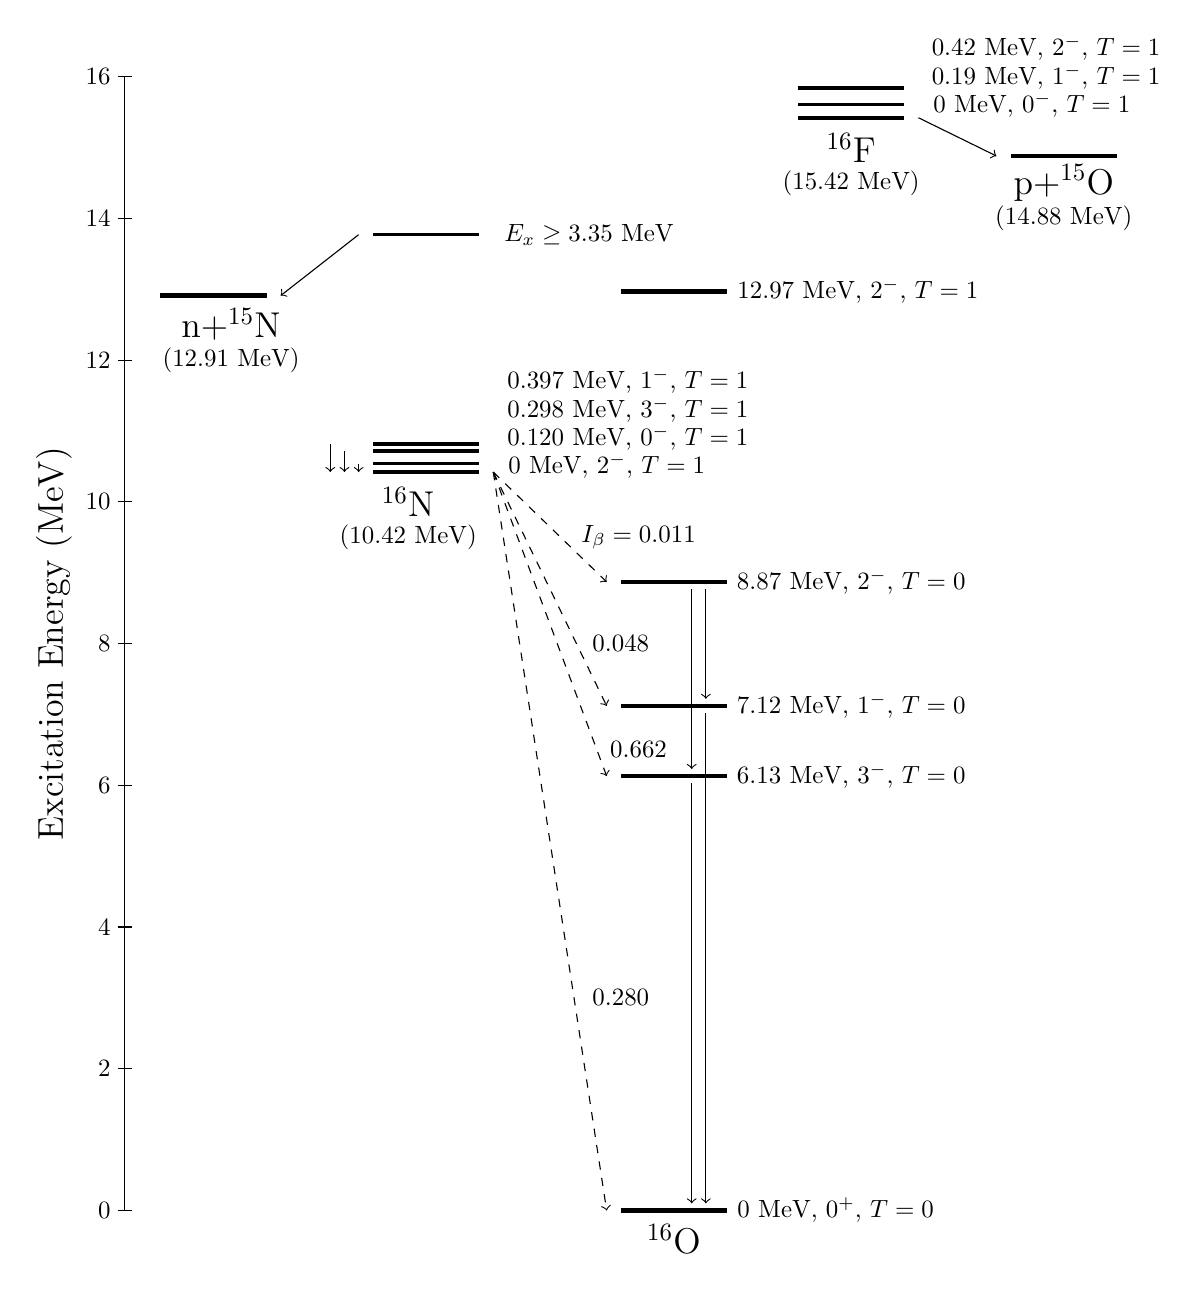
\begin{tikzpicture}[scale=0.9, every node/.style={scale=0.9}]
% Draw the energy axis
\draw (1,0) -- (1,16);
\node[rotate=90, font=\Large] at (0,8) {Excitation Energy (MeV)};
% Adding energy labels
\foreach \y in {0, 2, 4, 6, 8, 10, 12, 14, 16}
    \draw (0.9,\y) -- (1.1,\y) node[left=5pt] {\y};
% Draw the excitation levels for n+15N
\draw[->] (4.3,13.77) -- (3.2,12.91);
\draw[ultra thick] (1.5,12.91) -- (3,12.91);
\node[font=\Large] at (2.5,12.5) {n+$^{15}$N};
\node at (2.5,12) {(12.91 MeV)};
% Draw the excitation levels for 16N
\draw[very thick] (4.5,13.77) -- (6,13.77);
\node at (7.55,13.77) {$E_x \geq 3.35$ MeV};
\draw[very thick] (4.5,10.817) -- (6,10.817);
\draw[very thick] (4.5,10.718) -- (6,10.718);
\draw[very thick] (4.5,10.54) -- (6,10.54);
\draw[ultra thick] (4.5,10.42) -- (6,10.42);
\node at (8.1,11.7) {0.397 MeV, 1$^-$, $T=1$};
\node at (8.1,11.3) {0.298 MeV, 3$^-$, $T=1$};
\node at (8.1,10.9) {0.120 MeV, 0$^-$, $T=1$};
\node at (7.8,10.5) {0 MeV, 2$^-$, $T=1$};
\draw[->] (3.9,10.817) -- (3.9,10.42);
\draw[->] (4.1,10.718) -- (4.1,10.42);
\draw[->] (4.3,10.54) -- (4.3,10.42);
\node[font=\Large] at (5,10) {$^{16}$N};
\node at (5,9.5) {(10.42 MeV)};
\draw[dashed,->] (6.2,10.42) -- (7.8,8.87);
\draw[dashed,->] (6.2,10.42) -- (7.8,7.12);
\draw[dashed,->] (6.2,10.42) -- (7.8,6.13);
\draw[dashed,->] (6.2,10.42) -- (7.8,0);
\node at (8.25,9.5) {$I_\beta=0.011$};
\node at (8,8) {0.048};
\node at (8.25,6.5) {0.662};
\node at (8,3) {0.280};
% Draw the excitation levels for 16O
\draw[ultra thick] (8,0) -- (9.5,0) node[right] {0 MeV, 0$^+$, $T=0$};
\draw[very thick] (8,6.13) -- (9.5,6.13) node[right] {6.13 MeV, 3$^-$, $T=0$};
\draw[very thick] (8,7.12) -- (9.5,7.12) node[right] {7.12 MeV, 1$^-$, $T=0$};
\draw[very thick] (8,8.87) -- (9.5,8.87) node[right] {8.87 MeV, 2$^-$, $T=0$};
\draw[ultra thick] (8,12.97) -- (9.5,12.97) node[right] {12.97 MeV, 2$^-$, $T=1$};
\node[font=\Large] at (8.75,-0.4) {$^{16}$O};
\draw[->] (9.2,8.77) -- (9.2,7.22);
\draw[->] (9.2,7.02) -- (9.2,0.1);
\draw[->] (9,8.77) -- (9,6.23);
\draw[->] (9,6.03) -- (9,0.1);
% Draw the excitation levels for 16F
\draw[ultra thick] (10.5,15.42) -- (12,15.42);
\node[font=\Large] at (11.25,15) {$^{16}$F};
\node at (11.25,14.5) {(15.42 MeV)};
\draw[very thick] (10.5,15.61) -- (12,15.61);
\draw[very thick] (10.5,15.84) -- (12,15.84);
\node at (13.8,15.6) {0 MeV, 0$^-$, $T=1$};
\node at (14,16) {0.19 MeV, 1$^-$, $T=1$};
\node at (14,16.4) {0.42 MeV, 2$^-$, $T=1$};
% Draw the excitation levels for p+15O
\draw[->] (12.2,15.42) -- (13.3,14.88);
\draw[ultra thick] (13.5,14.88) -- (15,14.88);
\node[font=\Large] at (14.25,14.5) {p+$^{15}$O};
\node at (14.25,14) {(14.88 MeV)};
\end{tikzpicture}

\end{document}